\documentclass[tikz]{standalone}
\usepackage{graphicx} % Required for inserting images
\usepackage{tikz}
\usetikzlibrary{shadows}
\usepackage{xcolor}
\usetikzlibrary{backgrounds}

\usetikzlibrary {arrows.meta,automata,positioning,fit,calc}

\definecolor{ProcessStepBackground}{HTML}{FFFAF0}
\definecolor{IntermediateStateColour}{HTML}{949698}
\tikzstyle{InfinitesimalNode}=[circle,draw=none,inner sep=0pt,minimum size=0pt]
\tikzstyle{ProcessStepNode} =[fill=ProcessStepBackground,rounded corners]
\tikzstyle{IdleState} =[fill=yellow,rounded corners]
\tikzstyle{OutputState} =[fill=red,rounded corners]
\tikzstyle{InputState} =[fill=green,rounded corners]
\tikzstyle{IntermediateState} =[fill=IntermediateStateColour,rounded corners]
\tikzstyle{Source} =[fill=ProcessStepBackground,circle]
\tikzstyle{Sink} =[fill=ProcessStepBackground,circle]

\tikzset{
diagonal fill/.style 2 args={fill=#2, path picture={
\fill[#1, sharp corners] (path picture bounding box.south west) -|
                         (path picture bounding box.north east) -- cycle;}},
reversed diagonal fill/.style 2 args={fill=#2, path picture={
\fill[#1, sharp corners] (path picture bounding box.north west) |- 
                         (path picture bounding box.south east) -- cycle;}}
}

\tikzstyle{InputAndOutputState} =[diagonal fill={red}{green},rounded corners, drop shadow,draw ]

\begin{document}
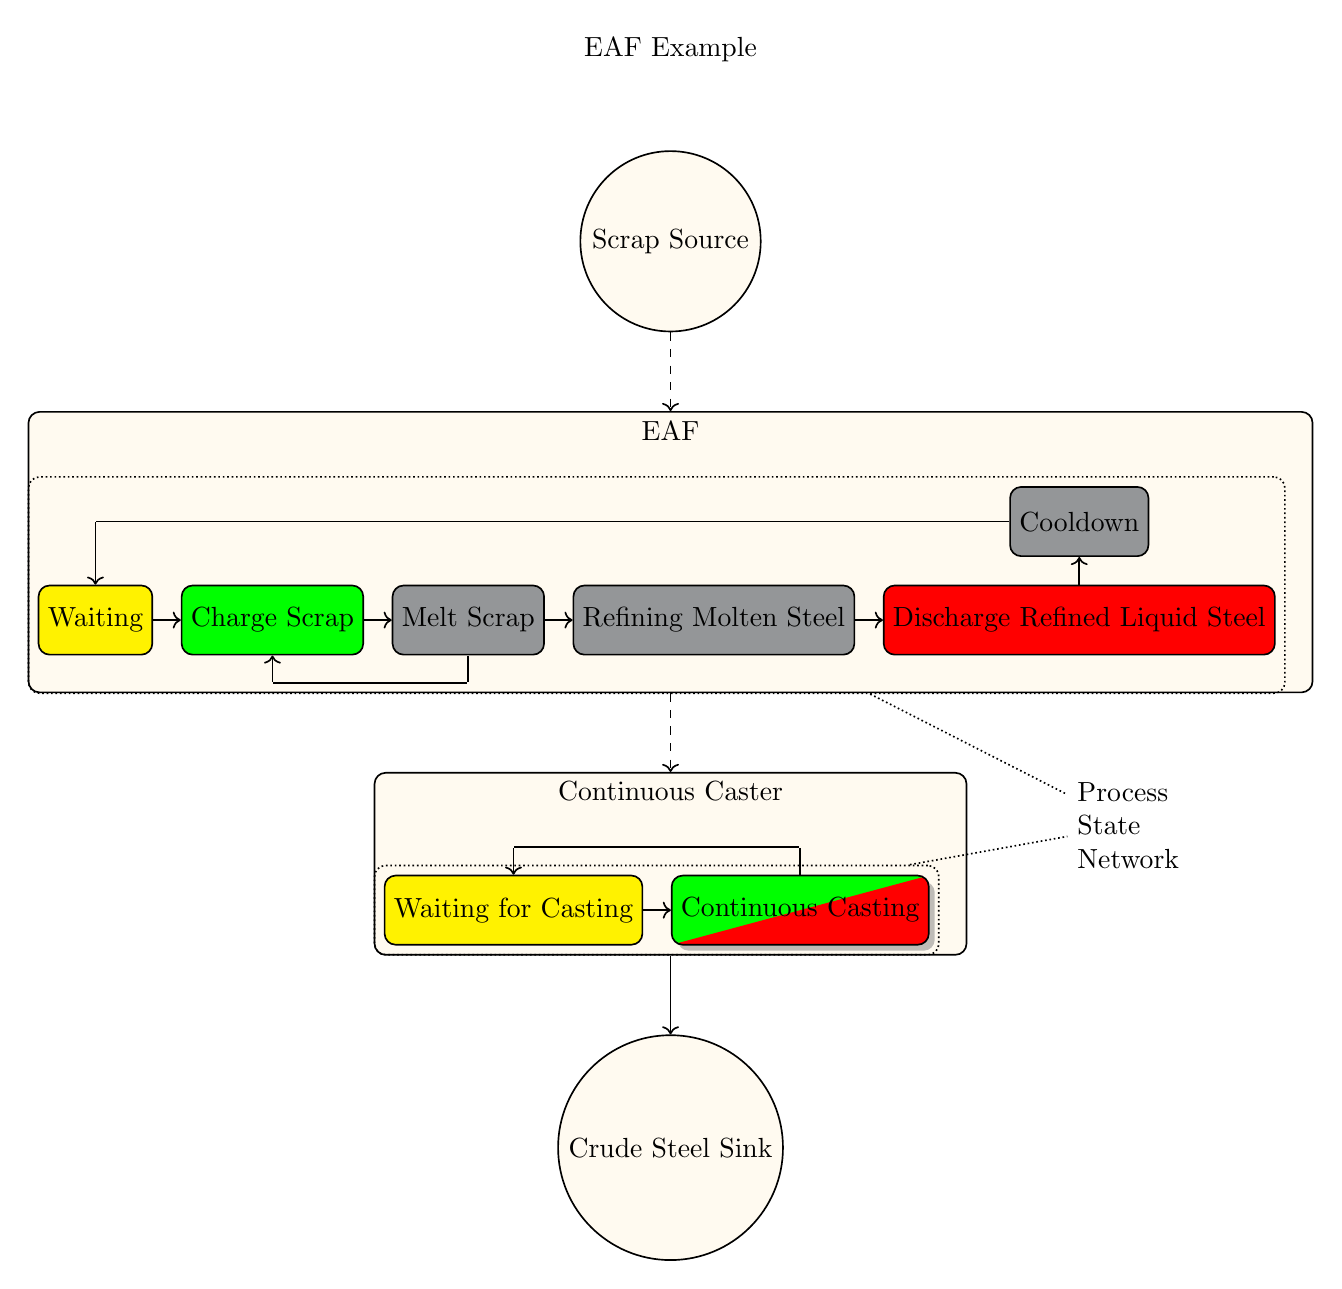
\begin{tikzpicture}[->,auto,node distance=1cm,on grid,semithick]
  \node[draw=none,rectangle](TitleNode){EAF Example};\node[draw,Source,below=of TitleNode.south](ScrapSource){Scrap Source};
  \matrix [column sep=10,row sep=10,draw,ProcessStepNode,below= of ScrapSource.south,rounded corners,nodes={rectangle, anchor=center}](EAF){
                                                                                                        &   & \node[text opacity=0]{B}; & \\
    \node[draw=none,InfinitesimalNode](f981de2e-cc7d-44ff-9756-e4526f3d33ae){};                         &
    \node[draw=none,InfinitesimalNode](801a230a-635c-4b66-9d7e-7bb64601f29f){};                         &
    \node[draw=none,InfinitesimalNode](ed81c651-575d-4320-8087-ee248f32932e){};                         &
    \node[draw=none,InfinitesimalNode](5728d4bf-c488-4333-99e7-b55ef568f2f1){};                         &
    \node[state,rectangle,IntermediateState](Cooldown){Cooldown};                                       &
    \\  \node[state,rectangle,IdleState](Waiting){Waiting}; &
    \node[state,rectangle,InputState](Charge-Scrap){Charge Scrap};                                      &
    \node[state,rectangle,IntermediateState](Melt-Scrap){Melt Scrap};                                   &
    \node[state,rectangle,IntermediateState](Refining-Molten-Steel){Refining Molten Steel};             &
    \node[state,rectangle,OutputState](Discharge-Refined-Liquid-Steel){Discharge Refined Liquid Steel}; &
    \\  \node[draw=none,InfinitesimalNode](b9cc9376-37e7-4ae6-aaff-15a35d29947a){}; &
    \node[draw=none,InfinitesimalNode](e058c9ca-4283-4be4-8fea-880e468cd84d){};                         &
    \node[draw=none,InfinitesimalNode](3462e6dc-1ad3-4332-875c-eda9d12207fe){};                         &
    \node[draw=none,InfinitesimalNode](f34780e4-c52e-4931-94bd-6bc5b91162aa){};                         &
    \node[draw=none,InfinitesimalNode](1d8d9712-610e-4dad-9b82-691ddd401f32){};                         &
    \\
  };


  \node[fit=(1d8d9712-610e-4dad-9b82-691ddd401f32)(Waiting)(Cooldown)(Discharge-Refined-Liquid-Steel),draw,rounded corners,densely dotted](ProcessStateNetwork1){};


  \node[below= 0 cm of EAF.north]{EAF};
  \draw[->] (Refining-Molten-Steel) -- (Discharge-Refined-Liquid-Steel);
  \draw[->] (Melt-Scrap) -- (Refining-Molten-Steel);
  \draw[->] (Charge-Scrap) -- (Melt-Scrap);
  \draw[->] (Waiting) -- (Charge-Scrap);
  \draw[<-] (Waiting) -- (f981de2e-cc7d-44ff-9756-e4526f3d33ae);
  \draw[-] (f981de2e-cc7d-44ff-9756-e4526f3d33ae) -- (Cooldown);
  \draw[<-] (Cooldown) -- (Discharge-Refined-Liquid-Steel);
  \draw[<-] (Charge-Scrap) -- (e058c9ca-4283-4be4-8fea-880e468cd84d);
  \draw[-] (e058c9ca-4283-4be4-8fea-880e468cd84d) -- (3462e6dc-1ad3-4332-875c-eda9d12207fe);
  \draw[-] (3462e6dc-1ad3-4332-875c-eda9d12207fe) -- (Melt-Scrap);
  \matrix [column sep=10,row sep=10,draw,ProcessStepNode,below= of EAF.south,rounded corners,nodes={rectangle, anchor=center}](Continuous-Caster){
                                                                                        & \node[text opacity=0]{B}; & \\
    \node[draw=none,InfinitesimalNode](ce50c9f0-a5d7-4918-b6f7-5438b82bf415){};         &
    \node[draw=none,InfinitesimalNode](01fa9030-f315-4d19-9ae2-e6f738052ffd){};         &
    \\  \node[state,rectangle,IdleState](Waiting-for-Casting){Waiting for Casting}; &
    \node[state,rectangle,InputAndOutputState](Continuous-Casting){Continuous Casting}; &
    \\
  };

  \node[fit=(Continuous-Casting)(Waiting-for-Casting),draw,rounded corners,densely dotted](ProcessStateNetwork2){};
  \node[below= 0 cm of Continuous-Caster.north]{Continuous Caster};
  \draw[->] (Waiting-for-Casting) -- (Continuous-Casting);
  \draw[<-] (Waiting-for-Casting) -- (ce50c9f0-a5d7-4918-b6f7-5438b82bf415);
  \draw[-] (ce50c9f0-a5d7-4918-b6f7-5438b82bf415) -- (01fa9030-f315-4d19-9ae2-e6f738052ffd);
  \draw[-] (01fa9030-f315-4d19-9ae2-e6f738052ffd) -- (Continuous-Casting);
  \node[draw,Sink,below=of Continuous-Caster.south](CrudeSteelSink){Crude Steel Sink};

  \draw[->,dashed](ScrapSource.south) -- (EAF.north);
  \draw[->,dashed](EAF.south) -- (Continuous-Caster.north);
  \draw[->](Continuous-Caster.south) -- (CrudeSteelSink.north);


  \node[below=of ProcessStateNetwork1.south east, draw=none,align=left,xshift=-2cm](ProcessStateNetworkLabel){Process\\State\\Network};

  \draw[-,densely dotted](ProcessStateNetwork1) -- (ProcessStateNetworkLabel);
  \draw[-,densely dotted](ProcessStateNetwork2) -- (ProcessStateNetworkLabel);


\end{tikzpicture}
\end{document}
